\documentclass[final,dvipsnames]{beamer}

% ====================
% Packages
% ====================

\usepackage[T1]{fontenc}
\usepackage{tgbonum}
\usepackage[size=a0,orientation=portrait]{beamerposter}
\usetheme{gemini}
\usecolortheme{mit}
\usepackage{graphicx}
\usepackage[justification=centering]{caption}
\usepackage{subcaption}
\usepackage{booktabs}
\usepackage{tikz}
\usetikzlibrary{trees, matrix, positioning, patterns, shapes, shadows, shapes.arrows, arrows.meta, shapes.multipart, decorations.pathreplacing, calc, tikzmark, shapes.geometric}
\usepackage{pgfplots}
\pgfplotsset{compat=1.14}
\pgfplotsset{every axis/.append style={very thick}}
\usepackage{pgf-pie}
\usepackage[binary-units]{siunitx}
\usepackage{anyfontsize}
\usepackage{amsmath}
\usepackage{mathdots}
\usepackage{mathtools}
\usepackage{listings}
\usepackage{xcolor}
\usepackage{bm}
\usepackage{ulem}
\newcommand{\soutthick}[1]{%
    \renewcommand{\ULthickness}{4pt}%
       \sout{#1}%
    \renewcommand{\ULthickness}{.4pt}% Resetting to ulem default
}
\newcommand{\soutverythick}[1]{%
    \renewcommand{\ULthickness}{8pt}%
       \sout{#1}%
    \renewcommand{\ULthickness}{.4pt}% Resetting to ulem default
}


% ====================
% Lengths
% ====================

% If you have N columns, choose \sepwidth and \colwidth such that
% (N+1)*\sepwidth + N*\colwidth = \paperwidth
\newlength{\sepwidth}
\newlength{\colwidth}
\setlength{\sepwidth}{0.025\paperwidth}
\setlength{\colwidth}{0.3\paperwidth}

\newcommand{\separatorcolumn}{\begin{column}{\sepwidth}\end{column}}

% ====================
% Title
% ====================

\title{\soutverythick{Safe}Tix, The Best-Worst QR-Code Ticketing system}

\author{ Julian Partanen \inst{1} \and Alexander Mattingley-Scott \inst{1}}

\institute[shortinst]{\inst{1} Heidelberg University}

% ====================
% Footer (optional)
% ====================

\footercontent{
	Beginners practical Binary Hacking 2024/25 \hfill
    \href{mailto:me272@uni-heidelberg.de}{me272@uni-heidelberg.de}, \href{mailto:tt249@uni-heidelberg.de}{tt249@uni-heidelberg.de}}
% (can be left out to remove footer)

% ====================
% Logo (optional)
% ====================

% use this to include logos on the left and/or right side of the header:
%\logoright{\includegraphics[height=6cm]{}}
%\logoleft{\includegraphics[height=6cm]{}}

% ====================
% Body
% ====================

\begin{document}

\begin{frame}[t, fragile]
\begin{columns}[t]
\separatorcolumn

\begin{column}{\colwidth}

    \begin{block}{About the original SafeTix}
        \begin{itemize}
            \item Ticketmaster is an American ticket sales and distribution company \cite{ticketmaster_wikipedia}
            \item For all kinds of events like concerts, sport events, theatre performances and more \cite{ticketmaster_wikipedia}
            \item Some partners: Taylor Swift, NFL, NHL, NBA, WWE, AEW, theatre productions like Harry Potter and the Cursed Child and many more \cite{ticketmaster_wikipedia}
            \item SafeTix: Rotating ticketing system by ticketmaster, initially introduced in 2019 \cite{introducing_safetix} \cite{ticketmaster_safetix_faq} \cite{nba_safetix_faq}
            \begin{figure}[h]
                \begin{center}
                    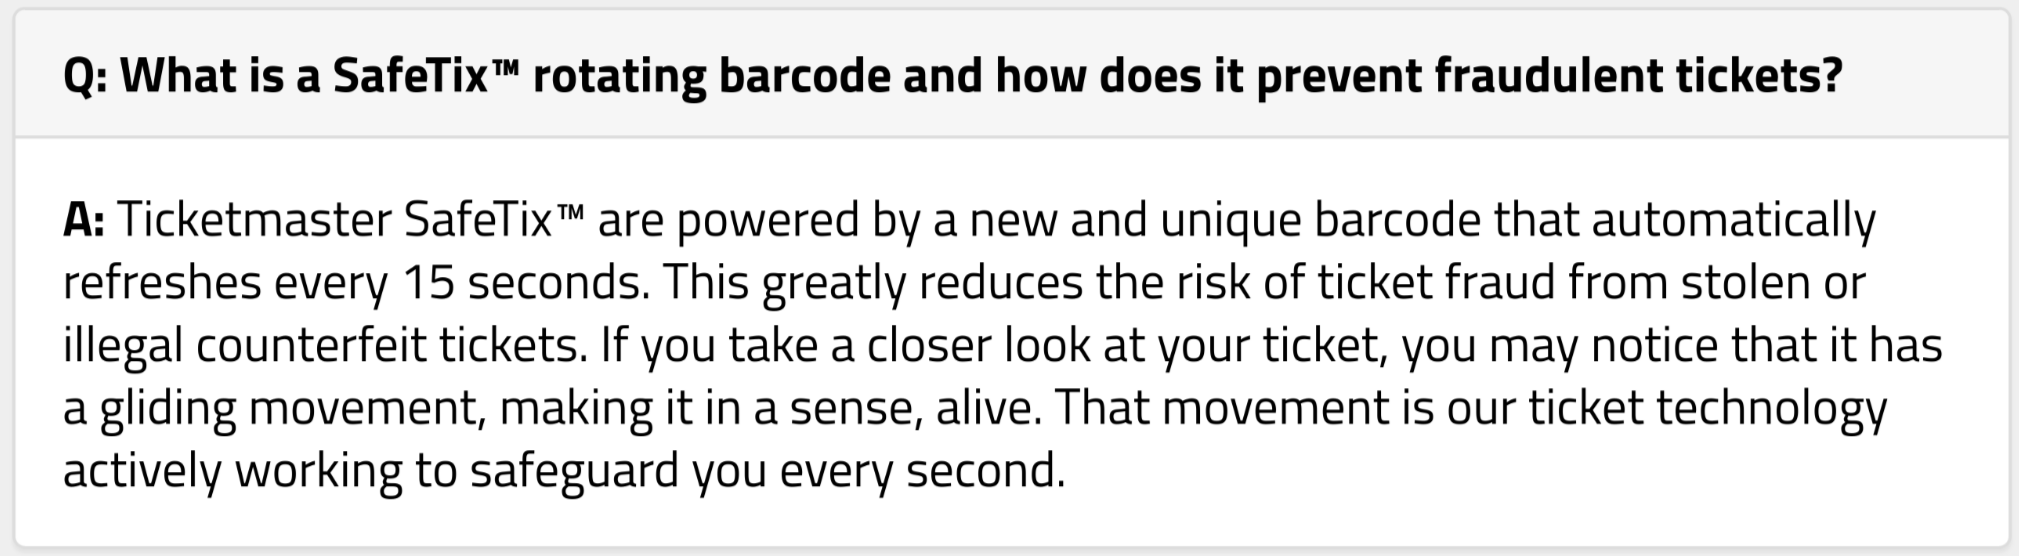
\includegraphics[width=\textwidth]{../figures/SafeTix_Quote_1.png}
                \end{center}
                \begin{center}
                    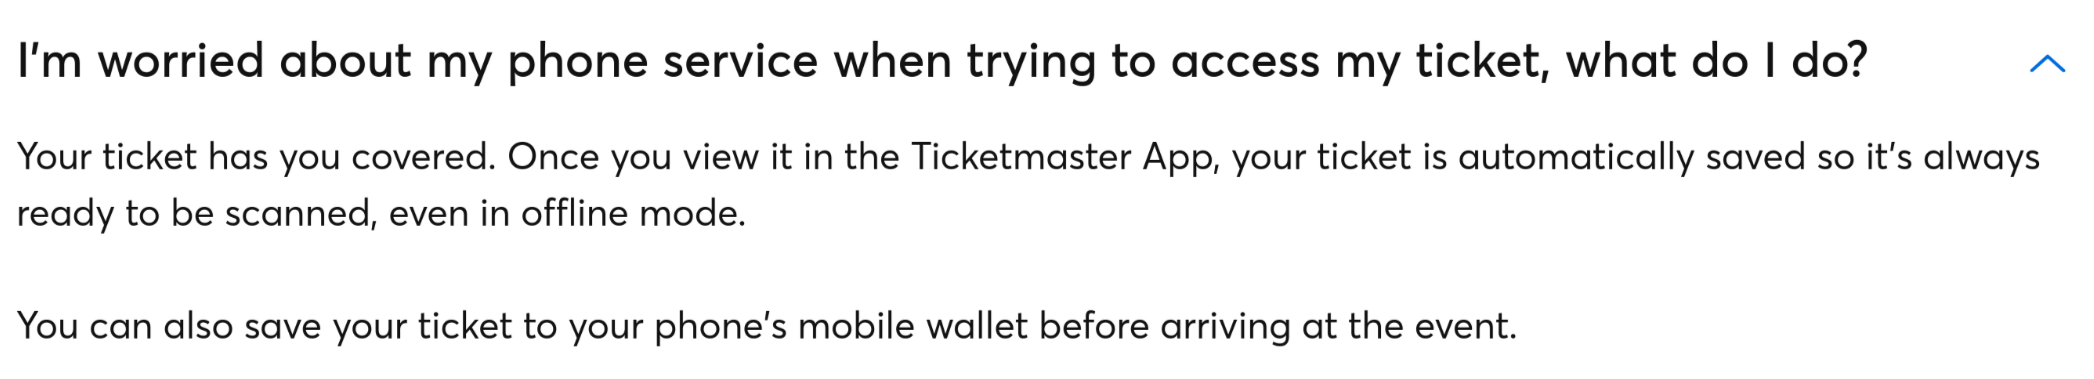
\includegraphics[width=\textwidth]{../figures/SafeTix_Quote_2.png}
                \end{center}
                \caption{Two quotes from ticketmaster's and NBA's FAQ pages about SafeTix \cite{ticketmaster_safetix_faq} \cite{nba_safetix_faq}}
                \label{fig:safetix_quotes}
            \end{figure}
            \item Barcode changes every 15 seconds, making transfers through screenshots or printouts impossible \cite{nba_safetix_faq}
            \item However ticket still works offline (once the ticket has been downloaded once) \cite{ticketmaster_safetix_faq}
        \end{itemize}

        \begin{figure}[htbp]
            \centering
            \begin{subfigure}[t]{0.45\textwidth}
                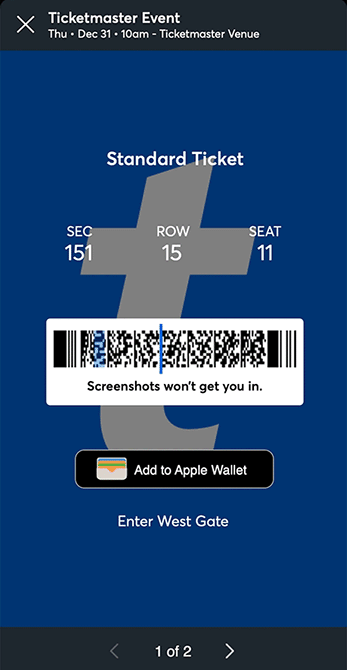
\includegraphics[width=\textwidth]{../figures/SafeTix_App_Barcode.png}
                \caption{A screenshot from ticketmaster's app showing SafeTix in action \cite{ticketmaster_mobile_ticketing}}
                \label{fig:app_barcode}
            \end{subfigure}
            \begin{subfigure}[t]{0.45\textwidth}
                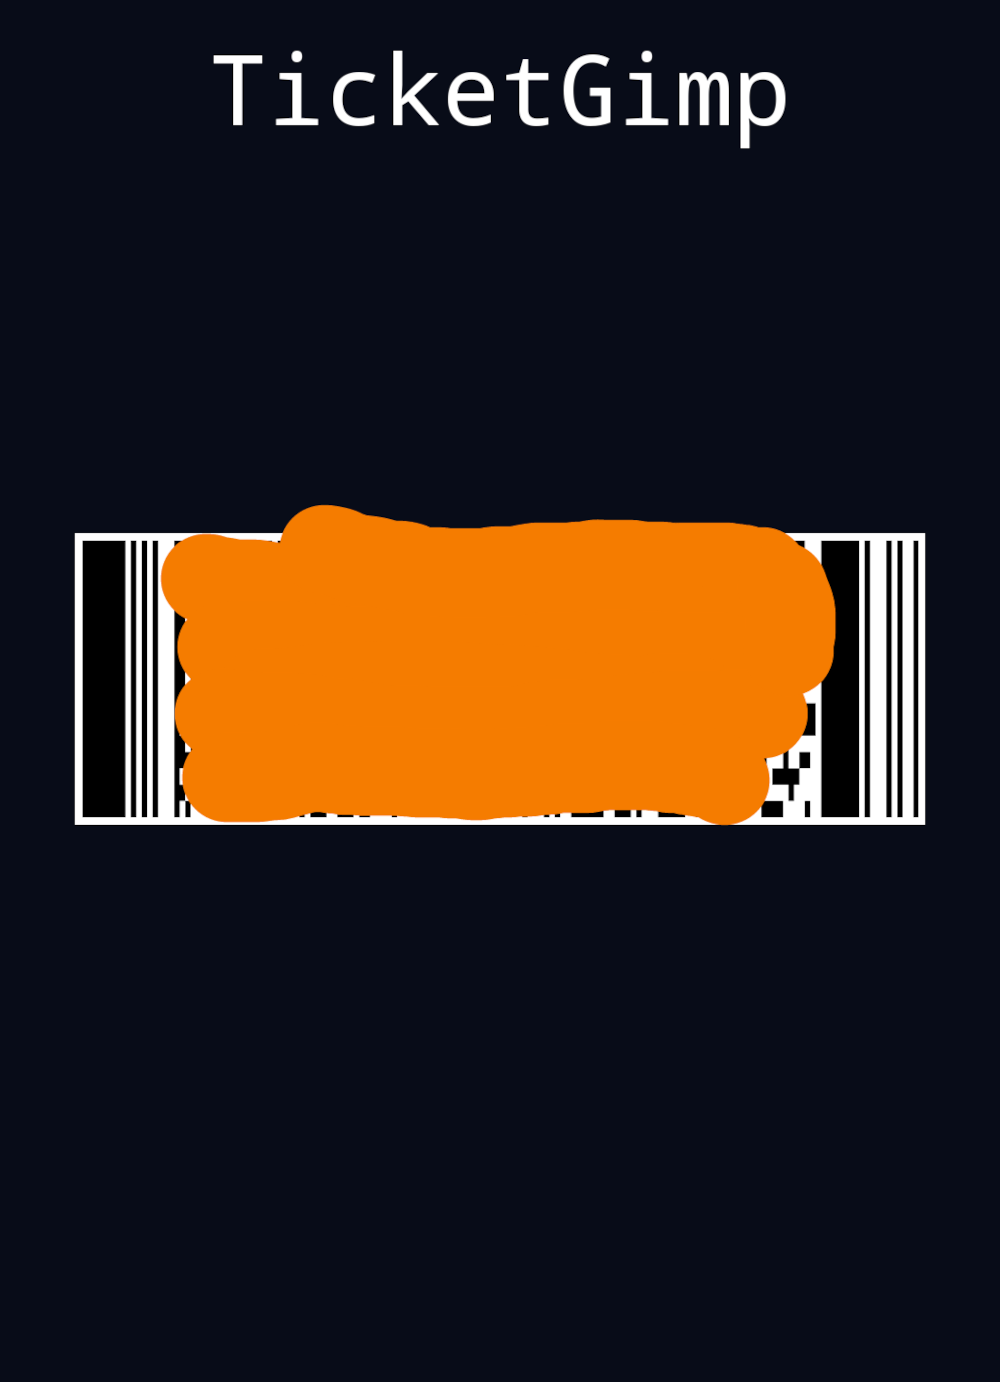
\includegraphics[width=\textwidth]{../figures/Conduition_custom_ticket_app.png}
                \caption{The Expo app TicketGimp Conduition wrote to store and render the extracted tickets \cite{reverse_engineering_ticketmaster}}
                \label{fig:conduition_custom_app}
            \end{subfigure}
            \caption{Official ticketmaster App vs. custom app for extracted tickets}
        \end{figure}
    \end{block}

    \begin{block}{How SafeTix got cracked}
        \begin{quotation}
            “Screenshots won’t get you in”, but Chrome DevTools will.
        \end{quotation}
        \begin{itemize}
            \item The Rust/Crypto developer Conduition reverse engineered SafeTix \cite{conduition}
            \item They managed to extract the ticket of ticketmaster's app into their own app and used that to enter the venue
            \item They described the process in a blog post \cite{reverse_engineering_ticketmaster}
            \item The barcode consists of a static bearer token and two rotating numbers \cite{reverse_engineering_ticketmaster}
            \item Rotating numbers: Standard TOTP (except only valid for 15 seconds instead of 30)
            \item TOTP secrets can be extracted from WebApp using either debug tools to analyse network traffic or by just reading the terminal output
        \end{itemize}
    \end{block}

    \begin{block}{References}
		%\nocite{*}
		\footnotesize{\bibliographystyle{ieeetr}\bibliography{poster.bib}}
	\end{block}

\end{column}

\separatorcolumn

\begin{column}{\colwidth}

    \begin{block}{Introducing: \soutthick{Safe}Tix, our binary hacking challenge}

		\begin{itemize}
			\item Our program is a recreation of the SafeTix application and consists of:
            
            \textbf{Server:}
            \begin{itemize}
                \item Written in \textbf{Python} using the \textbf{Flask} web framework
                \item Handles authentication, ticket issuing and ticket validation
                \item Each ticket is returned as an unique \textbf{ticket token} and \textbf{TOTP secret}
                \item \textbf{flask-JWT-extended} for user authentication, \textbf{pyotp} for generating TOTP secrets
                \item Deployment with \textbf{gunicorn} and custom bash script for \textbf{SSL}
            \end{itemize}
        
            \textbf{Client:}
            \begin{itemize}
                \item Written in \textbf{C++} (in contrary to original app which was a web app)
                \item \textbf{Qt} UI-framework and \textbf{qrencode} library for displaying QR codes in a window
                \item \textbf{cpp-httplib} and \textbf{nlohmann's json} libraries for communicating with the server
                \item \textbf{libcotp} library for generating one time passwords out of TOTP secret
                \item Regenerates QR codes every 15 seconds
                \item Bash script installs dependencies and compiles it
            \end{itemize}
            \begin{figure}[h]
				\centering
				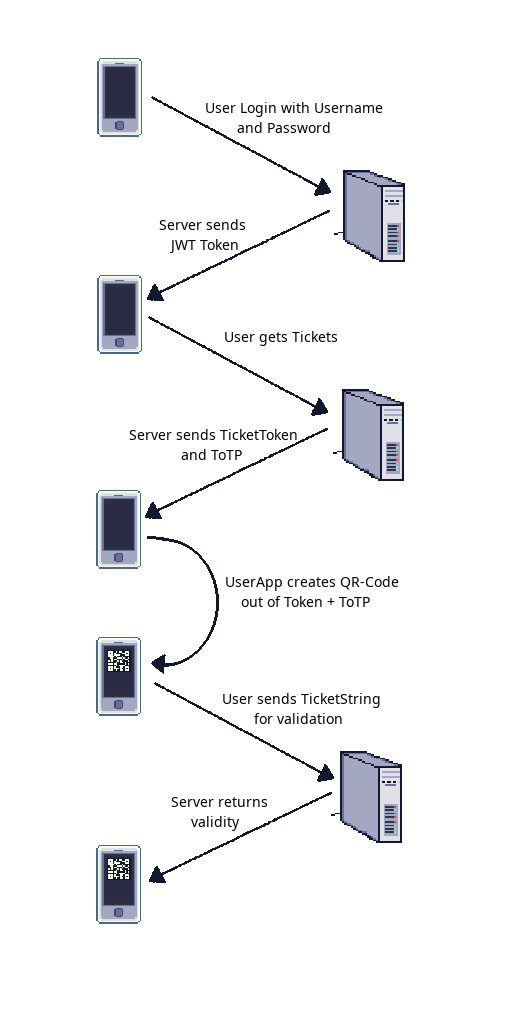
\includegraphics[width=0.8\textwidth]{../figures/Workflow_v2.png}
				\caption{Sequence diagram showing the communication between client and server}
				\label{fig:WorkFlow1}
			\end{figure}
            \begin{figure}[h]
				\centering
				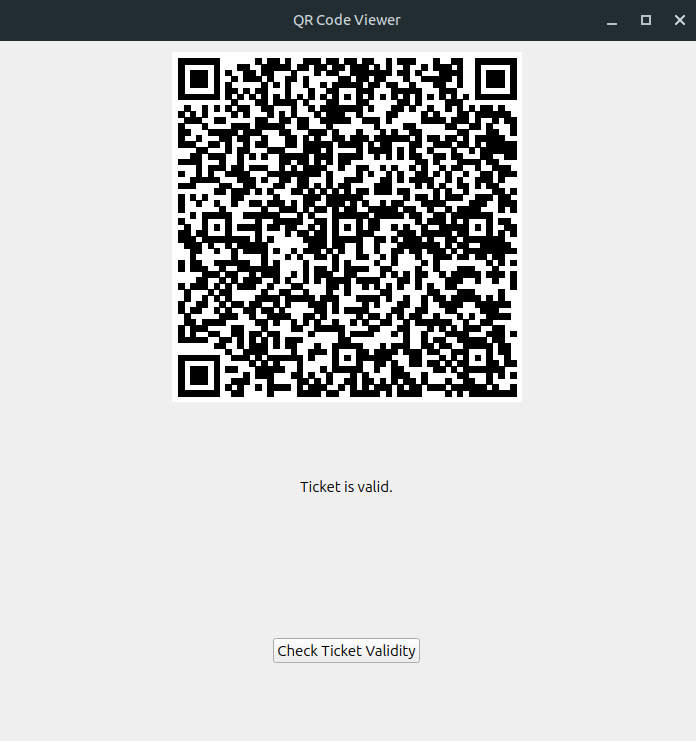
\includegraphics[width=0.7\textwidth]{../figures/QR_Window.png}
				\caption{Client window displaying the current ticket as a QR-code}
				\label{fig:WorkFlow1}
			\end{figure}
            \item By recreating SafeTix, we aimed to make it a notch safer (not logging the ticket to the console) but keep it "Reverse Engineerable"
            
            \item To solve the challenge, please follow this link to our Github repository and follow the instructions in the README:
            \begin{figure}
                \centering
                
\includegraphics[width=0.5\textwidth]{../figures/github_qr_code.png}
                \caption{https://github.com/JulianFP/unsafeTicks}
                \label{fig:GithubQRCode}
            \end{figure}
		\end{itemize}
	\end{block}

\end{column}

\separatorcolumn

\begin{column}{\colwidth}
    \begin{block}{How to Crack}
        \begin{figure}[h]
            \centering
            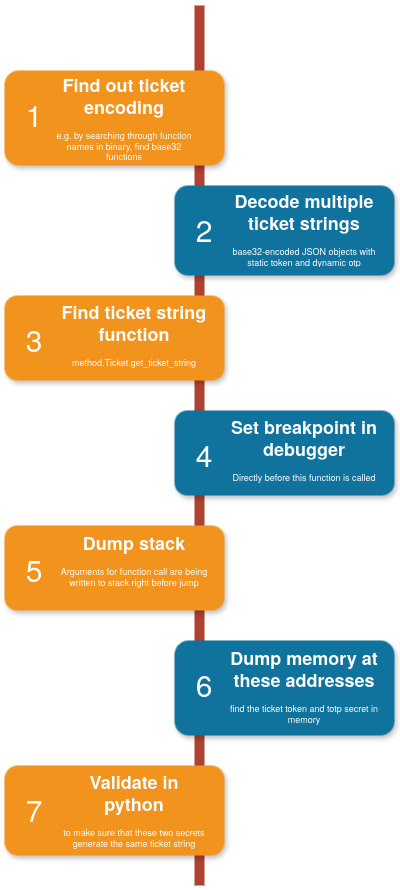
\includegraphics[width=0.7\textwidth]{../figures/HackingFlow.png}
            \caption{An example of how the ticket could be extracted from the program}
            \label{fig:HackingFlow}
        \end{figure}
        \begin{figure}[h]
            \centering
            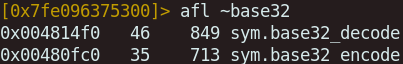
\includegraphics[width=0.7\textwidth]{../figures/Hacking_step_1.png}
            \caption{Step 1: Find base32 functions}
            \label{fig:HackingStep1}
        \end{figure}
        \begin{figure}[h]
            \centering
            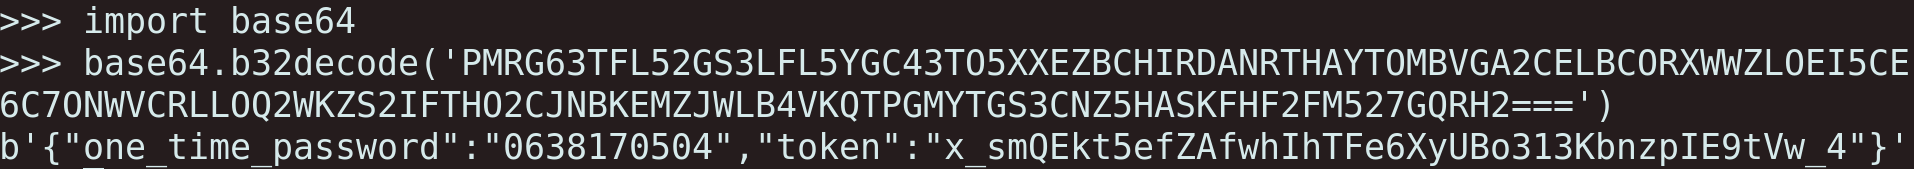
\includegraphics[width=0.95\textwidth]{../figures/Hacking_step_2.png}
            \caption{Step 2: Decode ticket string from QR-Code}
            \label{fig:HackingStep2}
        \end{figure}
        \begin{figure}[h]
            \centering
            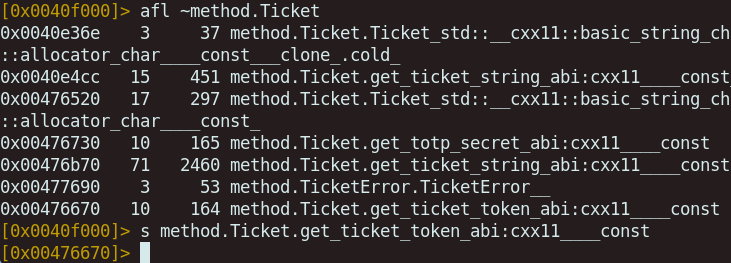
\includegraphics[width=0.95\textwidth]{../figures/Hacking_step_3.png}
            \caption{Step 3: Find the function that needs both the ticket token and the TOTP secret as an argument}
            \label{fig:HackingStep3}
        \end{figure}
        \begin{figure}[h]
            \centering
            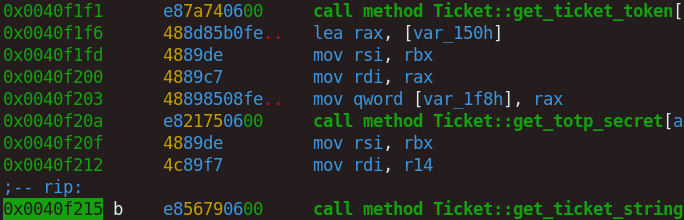
\includegraphics[width=0.95\textwidth]{../figures/Hacking_step_4.png}
            \caption{Step 4: Startup debugger and set breakpoint}
            \label{fig:HackingStep4}
        \end{figure}
        \begin{figure}[h]
            \centering
            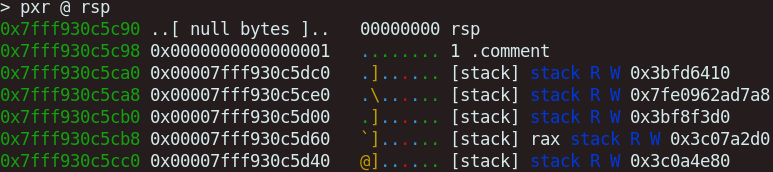
\includegraphics[width=0.95\textwidth]{../figures/Hacking_step_5.png}
            \caption{Step 5: Stack dump}
            \label{fig:HackingStep5}
        \end{figure}
        \begin{figure}[h]
            \centering
            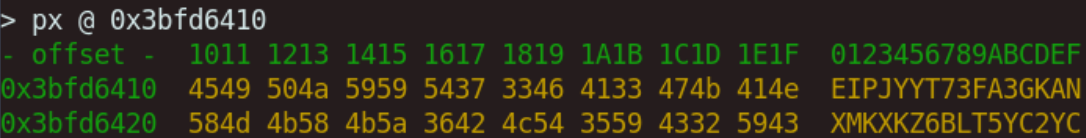
\includegraphics[width=0.95\textwidth]{../figures/Hacking_step_6.png}
            \caption{Step 6: Memory dump containing TOTP secret}
            \label{fig:HackingStep6}
        \end{figure}
        
    \end{block}
    \begin{block}{How to Improve}
        \begin{itemize}
            \item Using Digital Rights Management (DRM):
            \begin{itemize}
                \item DRM restricts offline access and prevents sharing/selling by enforcing restrictions like limiting the number of devices for a ticket.
                \item This improves the security but comes with less User friendliness.
            \end{itemize}
            \item Limit Offline Use:
            \begin{itemize}
                \item Restrict the ticket’s validity to a short period (e.g., 24 hours). 
                \item Reduces the window for resale but may be inconvenient for users.
            \end{itemize}
            \item Not Supporting Offline Tickets:
            \begin{itemize}
                \item Simply don't allow offline use at all.
                \item Will be very inconvenient for users.
            \end{itemize}
        \end{itemize}
    \end{block}
    

\end{column}




\separatorcolumn
\end{columns}
\end{frame}

\end{document}
